\documentclass[book.tex]{subfiles}
\begin{document}
\section{Source Code}
The game engine was released on July 21, 1995. 20 years later it is still there on the company ftp\footnote{Transfer File Protocol (along with Finger where J.C.Carmack used to blog) was commonly used in the 90s in the blessed time where you did not have to encrypt everything on the wire.}:\\ 
\\\codeword{ftp://ftp.idsoftware.com/idstuff/source/wolfsrc.zip}.\\
\\
\textbf{\underline{Trivia :}} Before the times of nmap, WireShark and various eavesdropping techniques, FTP\footnote{File Transfer Protocol} was commonly used to transfer files: It was simple and naively transmitted username and password in clear. Needless to say it did not age well...\\

\section{First Contact}
The file \codeword{woldsrc.zip} contains an other self-extracting PKZIP archive. It was a convenience back in the day but it is not practical nowadays. You can deflate it with:\\
\\\codeword{unzip WOLFSRC.1}.\\
\par
A few quick stats:\\
\begin{verbatim}
wolfsrc\$ cloc-1.64.pl .

      96 text files.
      94 unique files.                              
      27 files ignored.

---------------------------------------------------------------------
Language           files          blank        comment           code
---------------------------------------------------------------------
C++                   26           5750           6201          21169
C/C++ Header          42            802            660           3900
Assembly              10            669            732           2150
DOS Batch              1              1              0              4
---------------------------------------------------------------------
SUM:                  79           7222           7593          27223
---------------------------------------------------------------------
\end{verbatim}
The game engine is mostly C with a few ASM routines for optimized stuff and I/O.\\


 \begin{fancyquotes}
   We didn't have spell checkers in our editors back then, and I always had poor spelling.  The word "collumn" appears in the source code dozens of times.  After I released the source code, one of the emails that stands out in memory read:
 \bigskip \\
It's "COLUMN", you dumb @\#\$\% !\\
 \bigskip \\
\textbf{John Carmack - Programmer}
 \end{fancyquotes}
 
The archive actually contains more than just \codeword{.H} (headers) and \codeword{.C} (code) files. Also present are:
\begin{itemize}
\item \codeword{GOODSTUF.TXT} Two emails from fans demonstrating the success of the game: An ex-POW and a Microsoft employee.
\item \codeword{.ASM} Assembly optimized routines. Also contains  routines to access VGA and refresh screen.
\item \codeword{SIGNON.OBJ}: The startup screen showing the system characteristic (RAM, EMS, XMS, Joystick, SoundCards) was linked in the binary. Because that screen was showed before any sub-system was started. TODO: This should be a trivia.
\item \codeword{GAMEPAL.OBJ} Game palette. Hardcoded and linked in the executable for the same reason described previously.
\item \codeword{README} How to build. You can find a complete tutorial in the Annexe of this book.
\item \codeword{RULES.ASI} ???
\item \codeword{SV.EXE} ???
\item Many files resulting in a previous compilation attempt.
\end{itemize}







\section{The Big Picture}
The main system of the engine is its 3D engine. Which is not really 3D: Maps are designed in 2D dimensions (lattitude and longitude) and a 3D dimensional view is generated at runtime. In that sense, it could be called a pseudo-3D engine. The game is broken down in flat levels which are divided into areas and rooms by a grid-based pattern of walls and doors. The first level E1M1:\par
\begin{figure}[H]
  \centering
 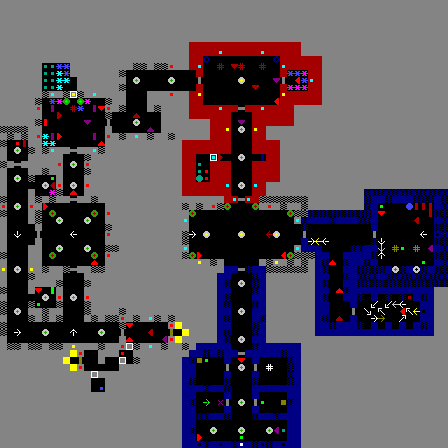
\includegraphics[width=\textwidth]{imgs/e1m1.png}
 \caption{The legendary E1M1 viwed from the top as in TED5 (Player is the green arrow at the bottom).}
\end{figure}
\par 


 \begin{figure}[H]
\centering
 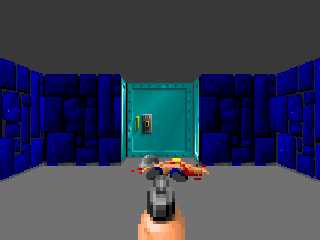
\includegraphics[width=\textwidth]{screenshots/wolf3d_7_fullframe.png}
 \caption{As it is rendered at runtime in pseudo-3D from the player point of view.} 
 \end{figure}


















\section{Architecture}

The engine is made of WL\_* files which relies on ID\_* sub-systems called Managers:
\begin{itemize}
	\item Memory
	\item Page
	\item Video
	\item Cache
	\item Sound
	\item User
	\item Input
\end{itemize}


\begin{figure}[H]
\centering
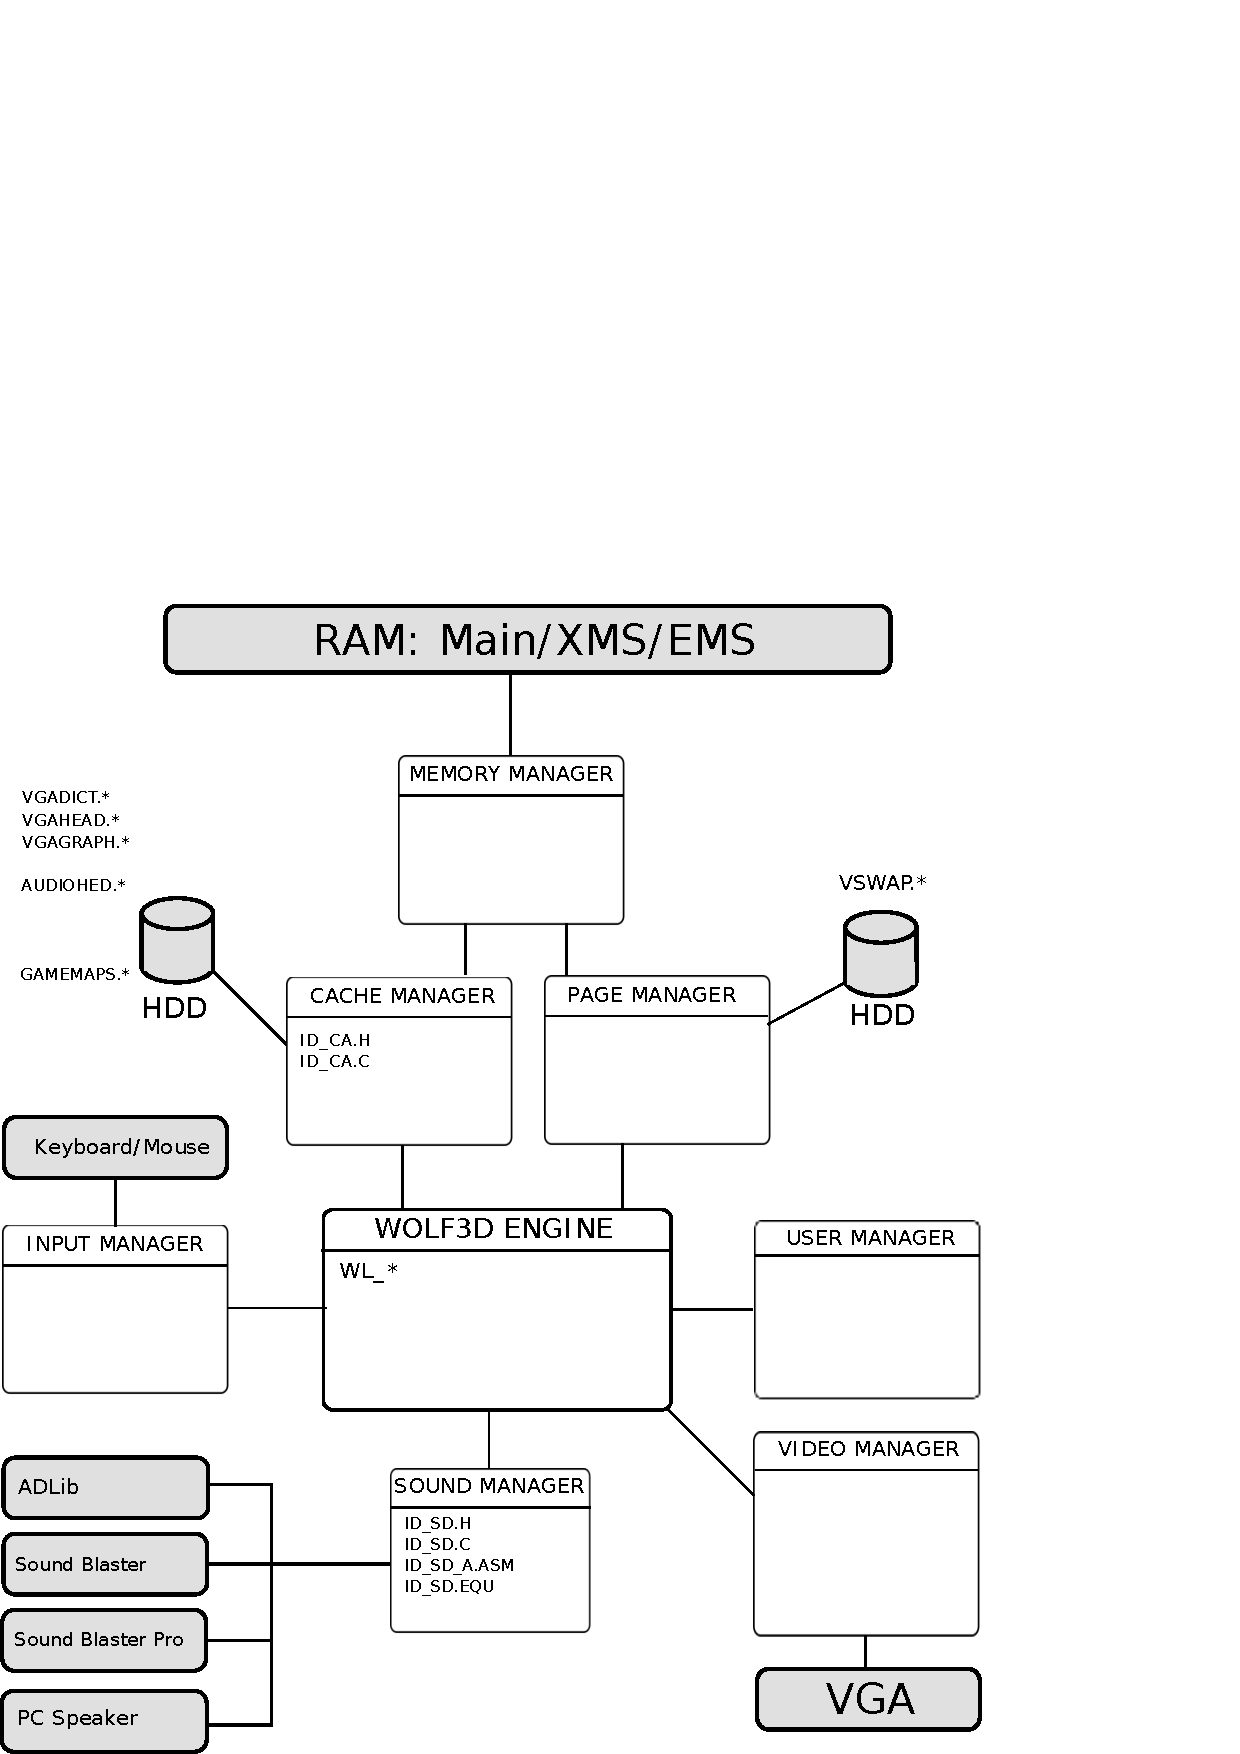
\includegraphics[width=\textwidth]{imgs/architecture.pdf}
\caption{Architecture with engine and sub-systems (in white) connected to I/O (in gray).}
\label{fig:architecture}
\end{figure}
Next to the hard drives (HDD) you can see the assets packed as described in the Team chapter.










\subsection{Memory Manager (MM)}
Harness the "fast" conventionnal memory.




\subsection{Page Manager (PM)}
The Page Manager harness the three types of RAM available: Conventional, XMS and XML. It abstract this complexity behind a Paging system.\\
Is it where the loading screen shows a progress bar ?
"Get Psyched !!!": Fill up the cache ?
Trivia: The progress bar was called a "thermometer".
The Page Manager provides all asset during 3D rendition. 
It loads as many "Pages" as possible in Main, XMS and EMS memory during the get Psyched screen.
TODO: Add a screenshot.
It uses a Least Frequency Used eviction policy if not all asset fit in RAM. VSWAP.WL6 is 1.6MB -> Recommended configuration 2MB RAM..but the game would run with just 640KB.


PAGE is for SWAP ! (see PML\_OpenPageFile)\\
According to the page header (Primary coder: Jason Blochowiak) Jason had experience with Unix programming and its design clearly is inspired of Unix SWAP file and paging system.
\subsection{Video Manager (VW)}


\subsection{Cache Manager (CA)}
The Cache Manager takes care of all the assets during Menu Phases: Sprites, Music, Sounds.
\subsection{Sound Manager (SD)}
The Sound Manager abstract interaction with all four sound systems supported: PC Speaker, ADLib (Music only), Sound Blaster (Mono), Sound Blaster Pro (Stereo).
\subsection{User Manager (US)}
Largely based on Catacom 3D code by Jason Blochowiak. Handles user. The copy/past is very visible since 90\% of the functions declared in the header (ID\_US.H) are not actually implemented in ID\_US.C. 

\subsection{Input Manager (IN)}
Abstract interaction with keyboard and mouse.























\section{Engine startup}
\subsection{MM (Memory Manager)}
Bla

\subsection{Video setup}
An important problem left open in the Hardware chapter, is the video card: None of the VGA modes available in the user manual are suited for a game engine. The most interesting one (13h) offers a single framebuffer of 256 indexed colors at a resolution of 320x200 with no square pixels (the 320x200 framebuffer was stretched to 320x240 on the screen). Nothing can be done about the non square pixels but there is something that can be done about the absence of double buffering.\\
\par
 In mode 13h, the VGA circuitry automatically maps the 16K adress space to the four VGA banks. It is called "chaining" and even though it wastes 75\% of the RAM it offers a linear framebuffer to the developer.\\
 \par
 Mode 13h is how the engine initialize the graphic pipeline:\\
\lstinputlisting[language=C]{code/init_vga.c}
 \par
\begin{figure}[H]
\centering
 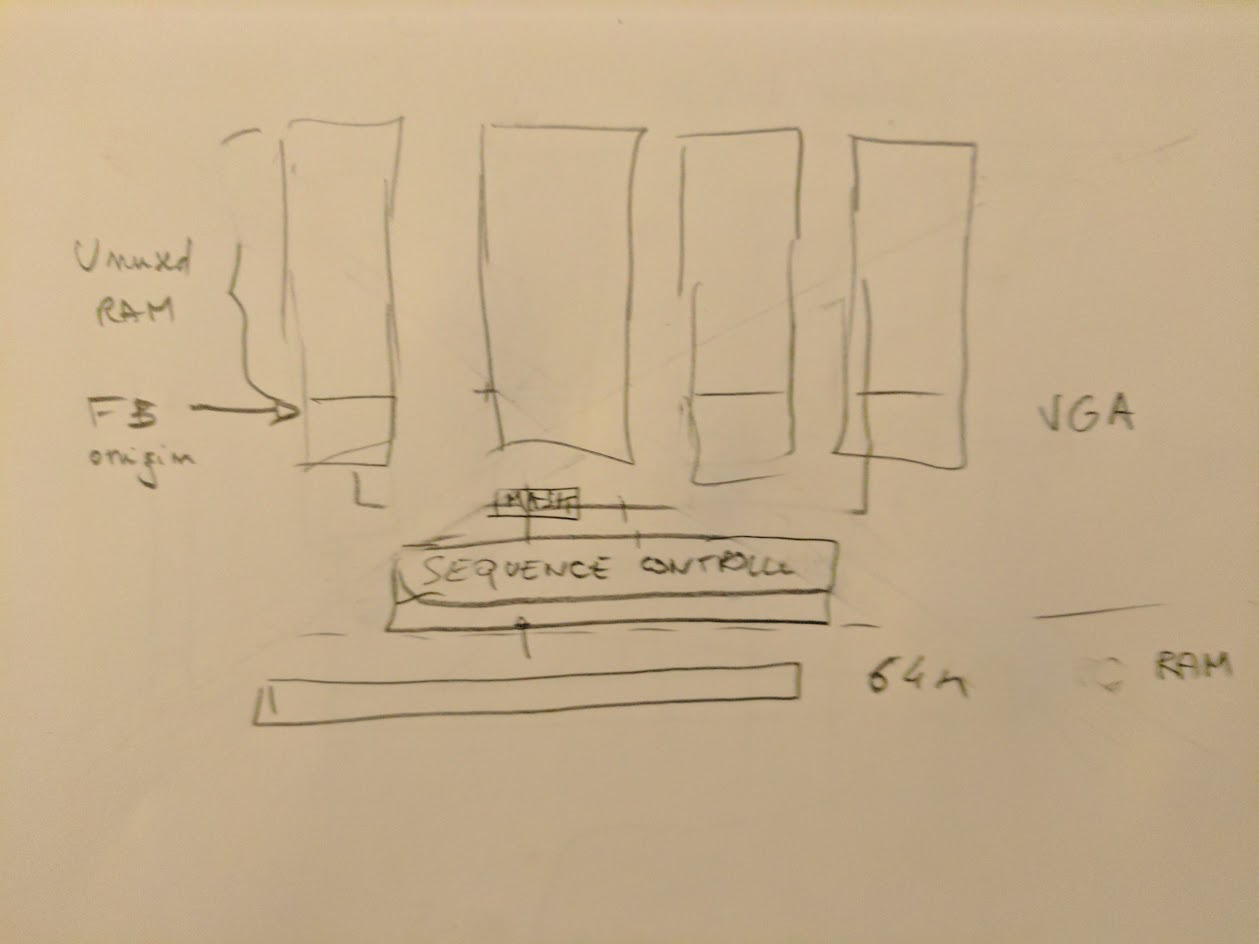
\includegraphics[width=\textwidth]{imgs/vga_layout/wasted_vga_ram.png}
 \caption{3D View as is appears on screen} \label{fig:vga_layout_in_3D}
 \end{figure}
 \par
 Even though it is undocumented in Mode 13h there is a way to disable chaining. Nobody can remember who invented unchaining but it was popularized by Michael Abrash\footnote{in Dr. Dobb's Journal} in July 1991. By tweaking the VGA Sequence controller the chaining can be disabled. The developer now has to manually drive the VGA mask to plot pixel but the full 256k of ram is available. This VGA mode is commonly called "Mode X". Note: In the engine, unchaining is called "deplane" in VL\_DePlaneVGA.
 \par
\lstinputlisting[language=C]{code//unchaining.c}
 \par
 To manually set the mask and select the bank were a value will be written can be done as follow
\lstinputlisting[language=C]{code//select_plan.c}
 \par
 With that much RAM available, wolf3d divides the VRAM in four parts:
 \begin{itemize}
 \item 64K for Framebuffer 0
 \item 64K for Framebuffer 1
 \item 64K for Framebuffer 1
 \item 64K for Graphic assets
\end{itemize}
\par
\begin{figure}[H]
\centering
 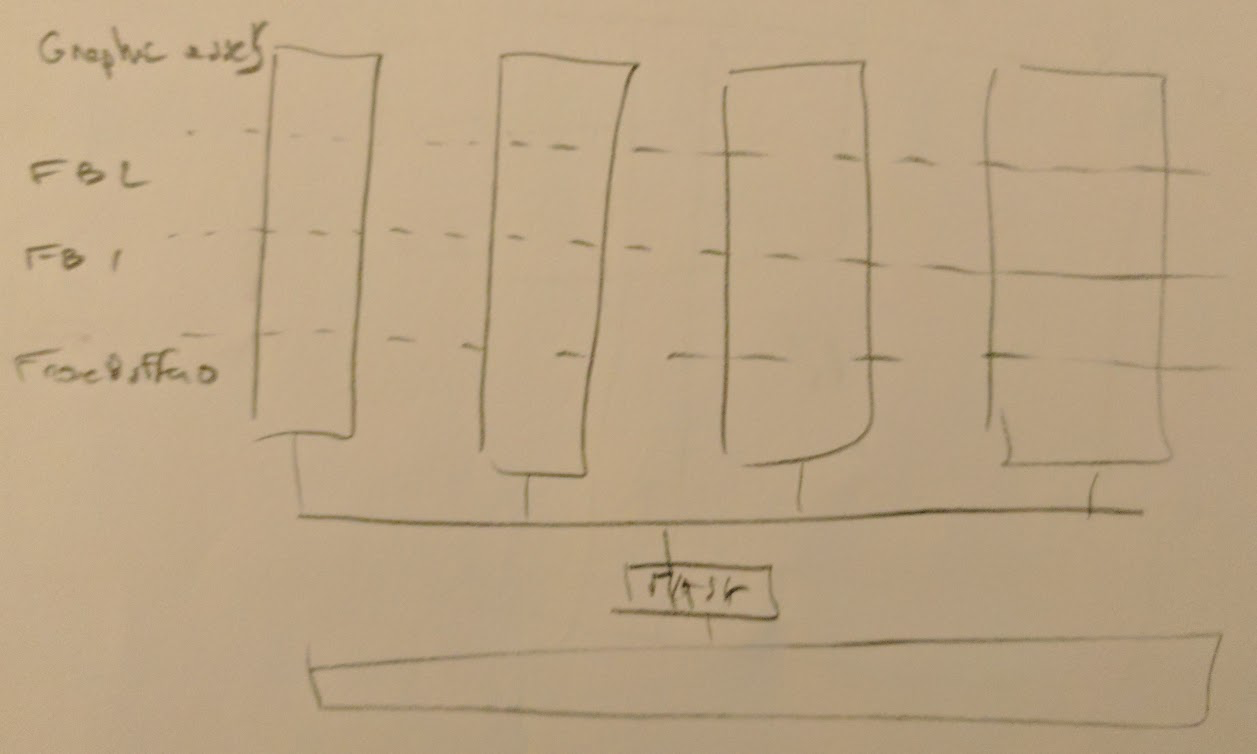
\includegraphics[width=\textwidth]{imgs/vga_layout/vga_ram_architecture.png}
 \caption{3D View as is appears on screen} \label{fig:vga_layout_in_3D}
 \end{figure}
As a result from unchaining a complete framebuffer is divided into four banks. Horizontally it looks a little bit like mashed potatoes:
 \begin{figure}[H]
\centering
 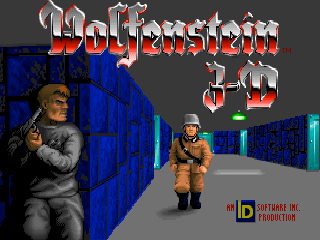
\includegraphics[width=\textwidth]{imgs/vga_layout/intro.png}
 \caption{Intro screen as it appear on screen}
 \end{figure}
 \par
 \begin{figure}[H]
\centering
 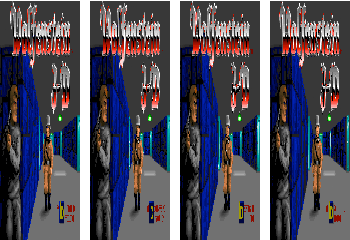
\includegraphics[width=\textwidth]{imgs/vga_layout/intro_bank.png}
 \caption{Intro screen as it is stored across 4 banks in a framebuffer} \label{fig:vga_layout_for_intro}
 \end{figure}
\par
An other example during a 3D sequence
\begin{figure}[H]
\centering
 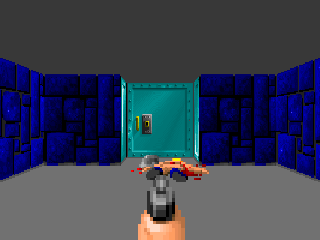
\includegraphics[width=\textwidth]{imgs/vga_layout/wolf3d_7.png}
 \caption{3D View as is appears on screen} \label{fig:vga_layout_in_3D}
 \end{figure}
 \par
 \begin{figure}[H]
\centering
 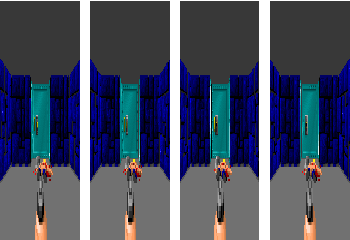
\includegraphics[width=\textwidth]{imgs/vga_layout/wolf3d_7_bank.png}
 \caption{3D View as it is stored across 4 banks in a framebuffer}
 \end{figure}

\par
But this solution only leads to an other problem. The automatic cicuitry of the VGA in Mode 13h is fast. Piloting manually the SC\_MASK is very slow. Therefore a naive algorithm drawing left to right and top to bottom as follow could not go beyond 4-5 frames per seconds:\\
\begin{verbatim}
void CleanScreen(y, color) {
  for(int y=0 ; y < 200 ; y++) {
    for(int x=0; x < 320 ; x++) {
      SelectBank(x % 4);
      WritePixel(x, y, color);   
    }
  }
}
\end{verbatim}\\
The culpit being the 320*200=64000 slow instruction to set the mask. But if we look carefully at the screenshot in Figure \ref{fig:vga_layout_for_intro} and Figure \ref{fig:vga_layout_in_3D} on page \pageref{fig:vga_layout_in_3D} there is an interesting propertly: Vertically the screen is still linear and not broken down in banks. This unlock different algorithm where things are drawn vertically:\\

\begin{verbatim}
void CleanScreen(y, color) {
  for(int x=0; x < 320 ; x++) {
    SelectBank(x % 4);
    for(int y=0 ; y < 200 ; y++) {
      WritePixel(x, y, color);   
    }
  }
}
\end{verbatim}\\
The previous code runs without issues at 70frames per second: Only 200 slow out instruction are used.\\
\par
This VGA bank layout has a fundamental impact on the engine: To draw anything fast, it has to be drawn \underline{vertically}. This hardware constraints has deep ramification in the engine: From the algotithms picked during 2D and 3D all the way up to the assets compression techniques.



\subsection{Signon}
At this point, the memory manager and the vga are initialized but nothing else. In order to make player wait for the rest of system to initialize, the engine displays the famous "PG13" screen (called in the engine "signon").
\begin{figure}[H]
\centering
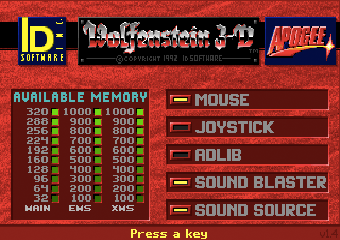
\includegraphics[width=\textwidth]{imgs/signon.png}
\caption{Architecture and sub-systems.}
\end{figure}
Since the graphic pipeline is not initialized at this point, the full 64K pg13 screen ships compiled in the executable. The engine only copies from RAM to the VGA banks. 
\lstinputlisting[language=C]{code/signonscreen.c}
Note: In an effot to get more RAM available, these 64K are unlinked for RAM.\\
Note: The palette (3*256=768B) is also compiled in the executable. It is simply copied from RAM to VGA's DAC.
Note the main (conventional memory) which goes only up to 320K: Between the exectuable and other residence routines it is all what was remaining of the original 640K. The game is able to run on 320KB but you needs to swap with the HD at runtime to load textures and sprites.



\subsection{Music and Heatbeats}
After showing something on screen, the audio and heatbeat system are started. This is done by reprogramming 8254-PIT and 8259-PIC timers to install an ISR\footnote{DOS Interrupt Service Routine}:\\
\begin{figure}[H]
\centering
 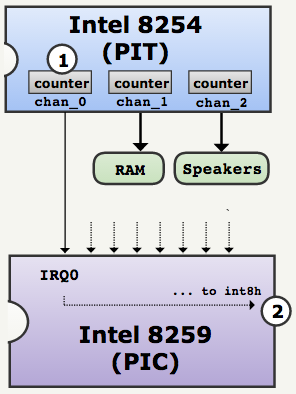
\includegraphics[width=\textwidth]{imgs/heatbeats.png}
 \caption{3D View as is appears on screen} 
 \end{figure}

Different things could happen depending on the hardware available:
\begin{itemize}
\item With the default PC speaker or with , the isr is set on slow: 140Hz
\item With an adlib or Disney Sound source, the isr is set on fast: 700Hz
\item With Sound Blaster, the isr is set on extreme: 7000Hz
\end{itemize}
Every time the ISR triggers, it takes care of feeding music and audio to the sound chip and also updates TimeCount variable, the heat of the whole system, at 70Hz (like VGA refresh rate).






\subsection{Profound Carnage}
The legendary "Profound Carnage-13" self-proclaimed rating, spoofing the movie industry PG-13 rating. Mark of the irreverent id software mindset at the time. Things like these would not fly these days.
\begin{figure}[H]
\centering

\includegraphics[width=\textwidth]{imgs/pg13.png}
\caption{Architecture and sub-systems.}
\end{figure}


\subsection{Menu phase}
\begin{figure}[H]
\centering
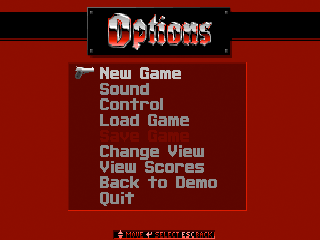
\includegraphics[width=\textwidth]{imgs/first_menu.png}
\caption{Architecture and sub-systems.}
\end{figure}

\end{document}